\subsection{Scoring Algorithm Test Runs}
These are the tests for the algorithms that help to score the quiz. The test generates a collection of fake answers, uses a brute force method to work out the score that these should be reduced down to, and then pipes them through the real algorithm - mimicking the ``stream'' of answers that would happen in production, whereby the final scores are calculated.

\subsubsection{housePoints.spec.js} % (fold)
\label{ssub:housepoints_spec_js}
\lstinputlisting[language=javascript, caption=Unit test for housePoints.js]{../test/housePoints.spec.js}
\begin{figure}[h!]
  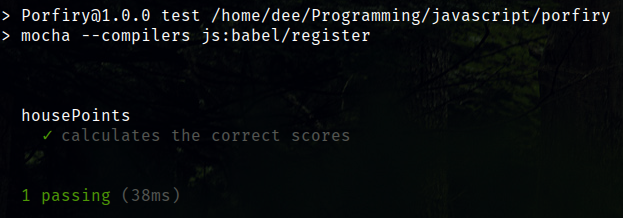
\includegraphics[scale=0.55]{testing/scoring/housepoints}
  \caption{Test outcome for housePoints.spec.js 1}
\end{figure}
% subsubsection housepoints_spec_js (end)

As is seen by the tick, the test passed successfully, meaning that the system is able to correctly calculate the winners of a quiz. \textit{Success.}
